In default setting of Hadoop, without setting the parameter "mapred.child.java.opt", a default setting with "-Xmx200M" will be transferred to tasktracker to use when start a child JVM for tasks. And the default setting for map tasks slot number is 2, which means the maximum running map tasks in task tracker is 2. A naive Hadoop users will never modify these configurations and maybe don't even know hadoop can be configured.
With default settings, Tasktracker will disable the TaskMemoryManagement Thread, so the only reason why the error message shows "Java Heap Size Error" is map task JVM use java heap to restore too much data, which is larger than the set 200MB.
We test with this setting of Hadoop with the customized wordcount described in section 4.1 which has four different types of memory behavior. Using Memmetric we monitor the memory behavior acted as we expected.

\begin{figure}[ht]
  \centering
    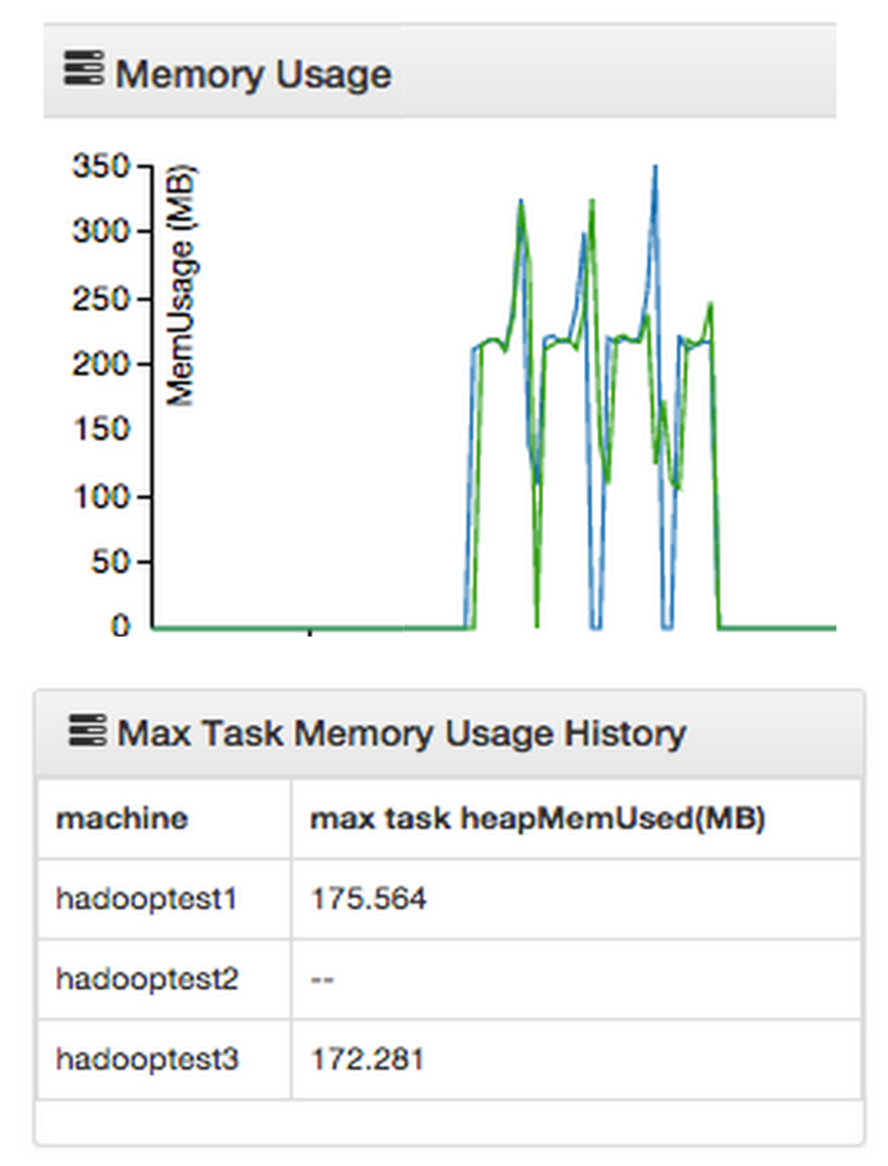
\includegraphics[width=2.1in]{image/test1a.png}
    \caption{Memory Usage under Same Threshold without Clearance}
    \label{ref:test1a}
\end{figure}

In Figure 13, the tested memory behavior is "Same Threshold without Clearance". The X-axis shows the time, and the Y-axis shows the memory usage with unit MB. The green line and blue line shows the sum of heap memory usage for all the tasks running on one slave machine (currently 2 tasks). The threshold is set to 200MB just the same with the configuration in JVM parameters. We can see from the figure that each line will increase the heap memory usage in exponential speed and then suddenly drop down to zero. And then due to failure, hadoop will start to rerun the task again on another machine, and we can see the increasing again, and after the sum is about 350MB, they are killed by the JVM as exceeding the maximum usage of JVM XMX setting. Then failure happens again, and restart again. We can also find the maximum value of heap usage for single task on one machine from the table, which shows almost 175MB. The reason why it just gets the value of 175MB but not some value bigger than 200MB is the exponential way of increasing data in holding, as everytime the arraylist add itself which doubles the data. So When it under 200MB, it will suddenly use too much memory, and killed by JVM itself, during which the process doesn't send out any metrics.

\begin{figure}[ht]
  \centering
    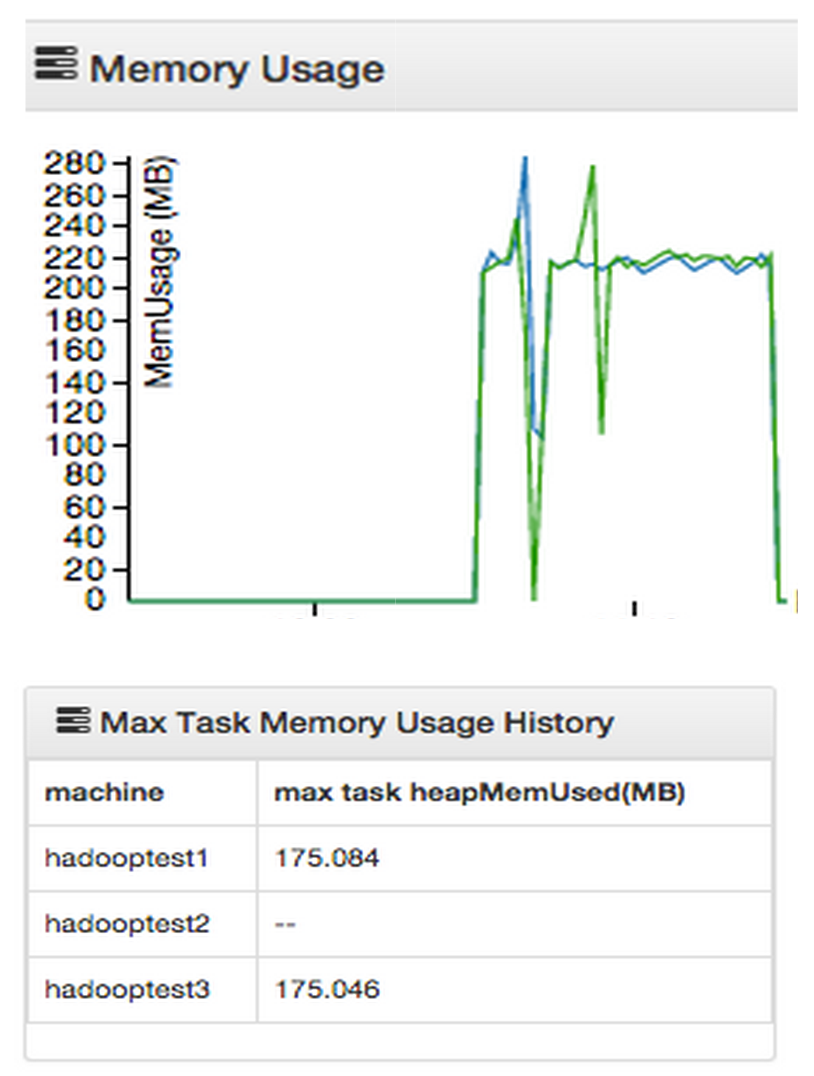
\includegraphics[width=2.1in]{image/test1b.png}
    \caption{Memory Usage under Random Threshold without Clearance}
    \label{ref:test1b}
\end{figure}

In Figure 14, the tested memory behavior is "Random Threshold without Clearance". We can find the lines are a little bit different with what shows in Figure 13. Some of the tasks keeps running without failure. That's the reason when the tasks fail of memory failure, the task is restarted with a random value that may decrease a lot the memory threshold. In this case, the retried task will run successfully. Even though in the maximum usage table, we can find the maximum usage is also about 175MB, but that is just the usage when fail happens.

\begin{figure}[ht]
  \centering
    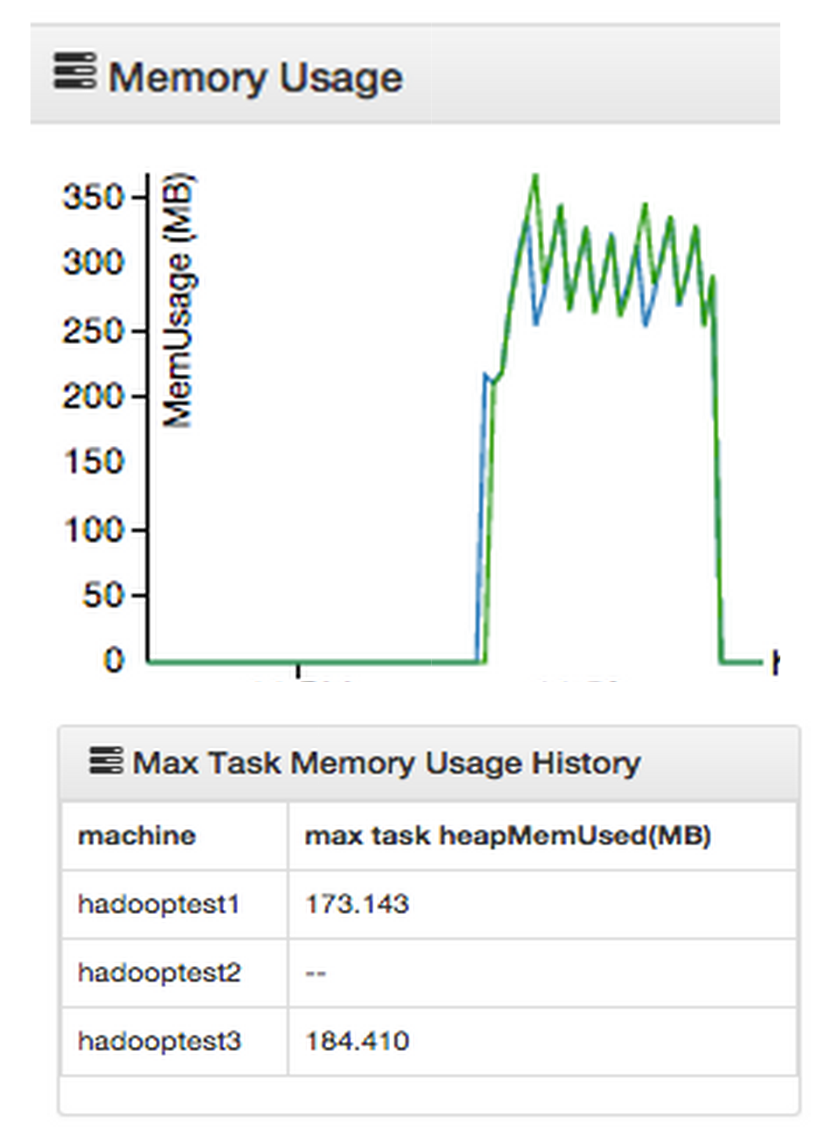
\includegraphics[width=2.1in]{image/test1c.png}
    \caption{Memory Usage under Same Threshold with Clearance}
    \label{ref:test1c}
\end{figure}

In Figure 15, the tested memory behavior is "Same Threshold with Clearance". We can find the tasks runs without any failure but much more unstable. As clearance will be triggered when the threshold is met. There are more big "Saws" in the graph.

\begin{figure}[ht]
  \centering
    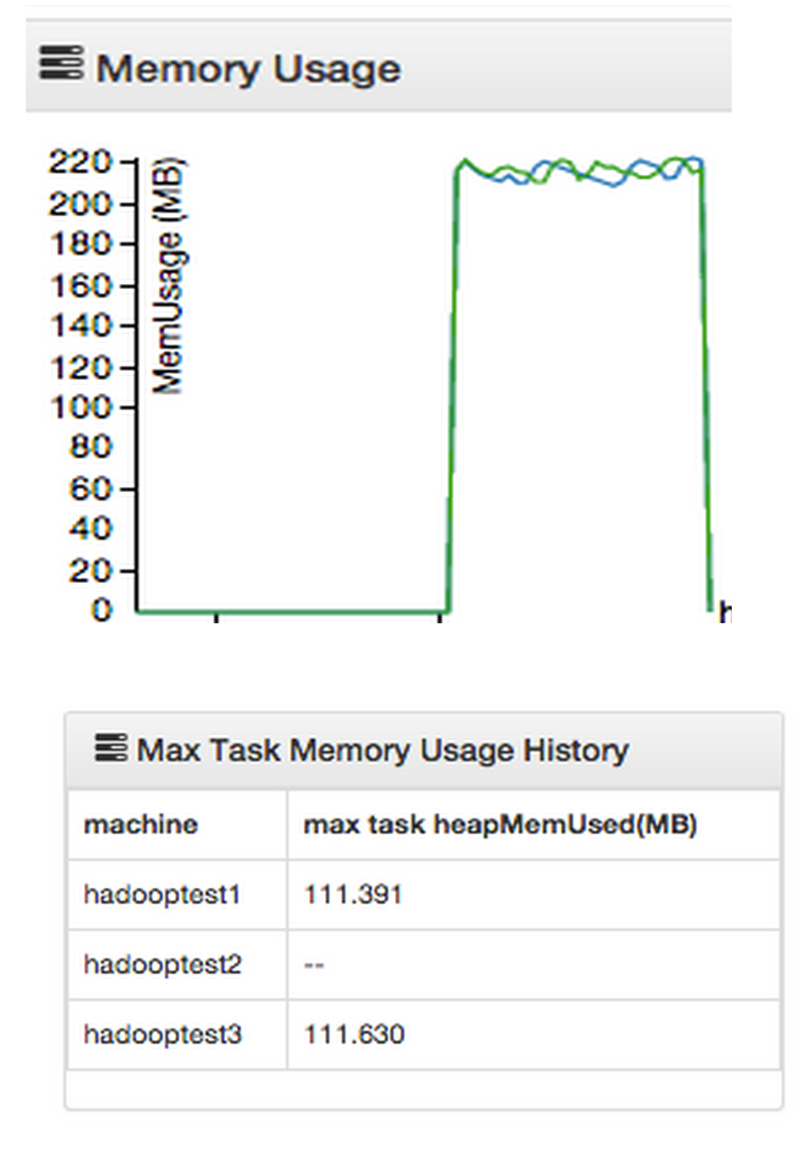
\includegraphics[width=2.1in]{image/test1d.png}
    \caption{Memory Usage under Random Threshold with Clearance}
    \label{ref:test1d}
\end{figure}

In Figure 16, the tested memory behavior is "Random Threshold with Clearance". In this case, the random threshold is about 110 MB, and it is always cleared after reach the threshold. So the green line and blue line is almost flat.
